\section{Introduction}
This chapter briefly presents in section \ref{sec:kundera} Kundera modular architecture, the way in which Kundera is supposed to be extended, the problems occurred in the process and how the community helped in achieving the result.

\noindent In section \ref{sec:develop} are discussed the detail of the two developed Kundera extension, in particular section \ref{sec:kundera-datastore} describe the extension for Google Datastore while section \ref{sec:kundera-table} the one for Azure Tables.

\section{Overview of Kundera}
\label{sec:kundera}
Kundera \cite{online:kundera} is an implementation of the JPA interface that currently supports various NoSQL datastore. It supports by itself cross-datastore persistence in the sense that its allows an application to store and fetch data from different datastores.
Kundera provides all the code necessary to implement the JPA 2.1 standard interface, independently from the underlying NoSQL database which is being used.

\newparagraph Currently supported NoSQL databases are:
\begin{itemize}
\item Oracle NoSQL (versions 2.0.26 and 3.0.5)
\item HBase (version 0.96)
\item MongoDB (version 2.6.3)
\item Cassandra(versions 1.2.9 and 2.0.4)
\item Redis (version 2.8.5)
\item Neo4j (version 1.8.1)
\item CouchDB (version 1.0.4)
\item Elastic Search (version 1.4.2)
\end{itemize}

\begin{figure}[tbh]
  \centering
  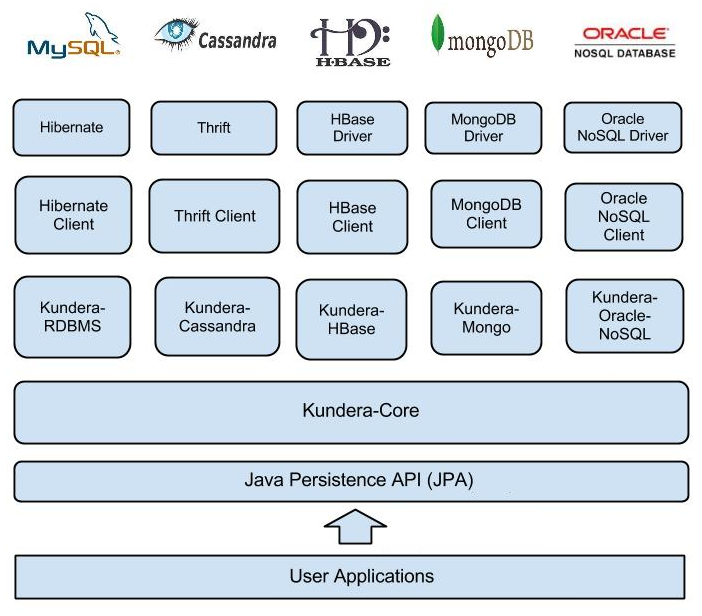
\includegraphics[scale=0.5]{images/kundera_architecture}
  \caption{Kundera architecture}
  \label{fig:kundera_architecture}
\end{figure}

\noindent The architecture of Kundera is shown in Figure \ref{fig:kundera_architecture}. The figure highlights the fact that the user application interacts with Kundera simply by exploiting the standard JPA interface implemented in the Kundera-Core.

\noindent Kundera-Core, each time an operation need to be executed on the underlying database, delegates the operation to the appropriate \texttt{Client} (creating it through a \texttt{Client Factory} if it does not exists yet). Clients are then responsible of actually executing the operation on the underlying database.

\subsection{Kundera's Client Extension Framework}
Kundera tries to offer a common way to interact with NoSQL databases through a well defined interface furthermore, since it is as on open source project, it makes other developers able to extend it, adding support for other databases.
The \textit{Client Extension Framework}, described in the Kundera documentation, provides a short description about how Kundera clients should work and gives a description of interfaces and classes that should be developed in order to make the client work properly.

\newparagraph Basically to build a new Kundera client, these are the blocks to be developed:
\begin{itemize}
\item the \texttt{Client}, which is the gateway to CRUD operations on database, except for JPQL queries and named queries;
\item the \texttt{Client Factory}, which is used by Kundera to instantiate the new Client;
\item the \texttt{Query implementor}, which is used by Kundera to run JPA queries by invoking appropriate methods in Entity Readers;
\item the \texttt{Entity Reader}, which is used by Kundera to translate the queries into correct client method calls;
\item optionally the \texttt{Schema Manager}, to support automatic schema generation.
\end{itemize}

\subsection{Approaching the extension}
While trying to extend Kundera we faced several problems that were not covered by the documentation, two were the main problem in understating what to do and how:
\begin{itemize}
\item when actually defined the classes and implemented the interfaces, it turns out that there are actually little differences both on interfaces and the required methods; 
\item the documentation lacks completely in describing what kind of information are carried by the argument of the methods that needs to be implemented.
\end{itemize} 

\noindent After getting the updated information from the community it turns out that the \texttt{Entity Reader} was unnecessary and all the translation from JPA queries to datastore specific queries and their executions should be done in the \texttt{Query Implementor}.  
Unfortunately no help was given by the community about the issue on methods arguments. Hence the most valid solution to approach the extension development was in a test driven way trying so to reverse engineer those arguments.

\section{Developing client extensions}
\label{sec:develop}
The work carried out has also focused on the development of two Kundera extensions, the first one for Google Datastore and the second one for Azure Tables.

\noindent Kundera \textit{Client Extension Framework} provides a generic interface which methods are supposed to carry out a lot amount of code, an example of this is the persist operation that is handled by the \texttt{onPersist} method, besides actually perform the persist operation, have to create an object that can be persisted by reading all the entity meta-data given as arguments and looking as example to relational fields.
\noindent The adopted solution is a template pattern in which each method maintains the main algorithm structure and delegates every operation to a specific hook method.
An example of this approach for the Datastore case, is reported in pseudo code in the snippet \ref{code:approach}.

\begin{lstlisting}[language=Java, caption=Template for the persist operation, label=code:approach]
@Override
protected void onPersist(...) {
    Entity gaeEntity = DatastoreUtils.createEntity(entityMetadata, id);
    handleAttributes(gaeEntity, entityAttributes);
    handleRelations(gaeEntity, relationHolders);
    handleDiscriminatorColumn(gaeEntity, entityMetadata);
    performPersist(gaeEntity);
}
\end{lstlisting}

\noindent For the Azure Tables extension, since it has been developed as the last one, the same structure has been kept and so it was only necessary to update the code of the hook methods.

\noindent The following sections presents these extensions separately, each feature developed is described in a dedicated section

\subsection{Google App Engine Datastore client}
\label{sec:kundera-datastore}
Google App Engine Datastore \cite{online:datastore} is the NoSQL solution build on top of Google BigTable a sparse, distributed, persistent multidimensional sorted map available in the App Engine platform. 

\subsubsection{JPA identifier}
The most basic unit that can be stored in Google Datastore is an \textit{Entity}, which is identified by a \textit{Key} and it is composed by \textit{Properties}.
Keys contain various information about the entity itself:
\begin{itemize}
\item the entity \textit{Kind}, which is used to group entities of the same type;
\item an entity identifier, used to distinguish entities of the same type;
\item an optional parent entity .
\end{itemize}
Inspired by the Google JPA implementation for Datastore \cite{online:googlejpa} the idea was to use the Java class representing the datastore \textit{Key} as identifier for the entity, but, unfortunately, this was not possible since Kundera support only a pre-defined defined set of Java data types.

\noindent Hence the adopted solution is to handle the key internally. Each time an operation on Datastore is required the key, relative to the entity, is built. The \textit{Kind} is directly mapped to the table name and the Key identifier is the user defined id specified in the \texttt{@Id} annotation.
The \texttt{@Id} annotation, in fact, is the annotation (available in the JPA specification) that is used to identify the class field that will be used as primary key in the resulting table on the underlying database.

\newparagraph IDs can be specified by the user or automatically generated, and they can be associated to three different data types
\begin{itemize}
\item \texttt{@Id} annotation on a \texttt{String} type field
\item \texttt{@Id} annotation on a \texttt{Long} type field
\item \texttt{@Id} annotation on a primitive \texttt{long} type field
\end{itemize}

\noindent Since Kundera supports the JPA feature for auto-generated IDs by using the annotation \texttt{@GeneratedValue}, this possibility has been exploited also for Datastore and so the user can annotate a \texttt{String} ID field so as that it will be auto-generated and its value will be a string representation of a random java \texttt{UUID}.

\noindent Auto-generated IDs are supported by Kundera only with \texttt{AUTO} or \texttt{TABLE} strategy, it was not possible to use the Datastore API to generate IDs since it is necessary to know the \textit{Kind} of the entity to be persisted but neither the \texttt{AUTO} strategy nor the \texttt{TABLE} one provides this information at generation time.

\subsubsection{Consistency}
In Datastore entities are organized in \textit{Entity Groups} based on their \textit{Ancestor Path}. The Ancestor Path is a hierarchy of entities whose keys have relation among themselves.

\noindent Consistency is managed through entity groups and so by defining the ancestor paths. Entities within the same entity group are managed in a strong consistency. Entities which are not in an entity group are treated with eventual consistent policy.

\noindent Datastore allows to create ancestor paths by defining entities parental relationships between entities and is it a task left to the user. Datastore low-level API also leave this task to the user, for example in Objectify \cite{online:objectify}, a wrapper for these API, the developer makes use of a \texttt{@Parent} annotation to make the user able to specify the parent relationships and hence to be able to organize entities through the ancestor path.

\noindent Since JPA is a well defined standard, adding such kind of annotation will break the standard and the only alternative left is trying to automatically guess the ancestor path.

\noindent An approach to do so can be to look at JPA relationships since they are clearly a good place to found information for guessing if two entity kind can be hierarchically related, hence for each type of relation we may define some solutions that can be adopted:
\begin{itemize}
\item for \textbf{One to Many} and \textbf{One to One} relationships, since there is an owning side of the relationship, the owning entity can be used as parent for every related entity. 
\item \textbf{Many to One} relationships can be considered as \textbf{One to Many} relationships. 
\item as regards \textbf{Many to Many} relationships, a solution can be to persist the elements of the join table as child of the entity in the owning side of the relationship but the specular solution (persist elements as child of the entity on the non-owning side) can be adopted too. The only solution that is not acceptable in this case is to persist both the entity, the one on the owning side and the one on the non-owning side, as parent to an element of the join table. This is principally due to the fact that this will require, as pointed out later, the Key of the join table element to be able to retrieve from Datastore the entities.
\end{itemize}

\noindent Even though it could have been possible to infer such relationships we choose not to implement it inside the Kundera extension for two main reasons: 
\begin{enumerate}
\item entities are not require to have a single relationship so, for example, if an entity contains two different relationships of type \textit{One to One} there is no way to decide which one should be used. Is so impossible, unless asking to the user, to decide which relation use to hierarchically organize entities
\item entities with a parent require, beside their own Key, the parent Key (and thus its Kind and identified) to be universally identified. For how Kundera is structured those information are not available and even if the parent entity Kind can be retrieved from Kundera meta-data, searching in the relationships meta-data, its identifier is not available inside meta-data as thus, since the complete Ancestor Path cannot be built, the entity cannot be retrieved. 
\end{enumerate}
\noindent For those reasons it was not possible to automatically guess ancestor paths by means of JPA relationships or make the user able manage them directly through a specific annotation without causing errors.
Each Kind is persisted as a root Kind hence each entity is stored as a separated entity group identified by its own Kind (the name of the JPA table associated to the entity).

\subsubsection{JPA relationships}
All the JPA supported relationships have been implemented in the client as it would have been done in a relational database.
So for \textbf{One to One} and \textbf{One to Many} relationships, on the owning side of the relationship, a \textit{reference} to the non-owning side entity is saved.

\noindent For \textbf{Many to One} relationships there would be two solutions:
\begin{itemize}
\item to persist a list of \textit{references} to the related entities;
\item not to persist anything within the entity and fill the relationship with a query.
\end{itemize}
The second solution has been adopted since it is more consistent with other Kundera client implementation and with the classic implementations (as well as relational databases client implementations).

\noindent As regards \textbf{Many to Many} relationships a join table is created based on user directives specified by means of the entity class annotations. The join table is filled each time a many to many related entity is persisted and a new \textit{row} is created inside the join table with the \textit{references} to the entities involved in the relationship.

\noindent The so far called \textit{reference} for Datastore is exploited by persisting within the entity the Key (Kind and identifier) of the related entity.

\newparagraph Can be useful at this point to show how an entity, annotated with the JPA standard, is then mapped to a datastore entity. 
Let's take as example the case described in the code \ref{code:entity-mapping}, the \texttt{Employee} class is annotated with many JPA annotations.
\begin{itemize}
\item the \texttt{@Entity} annotation specify to the JPA provider that this will be mapped to an entity in the underlying database and the \texttt{@Table} annotation specify the name that the table should have and the persistence unit to which the entity refer;
\item the \texttt{id} field will handle the identifier for this entity as it is annotated with the \texttt{@Id} annotation and furthermore this id will be auto-generated due to the presence of the \texttt{@GeneratedValue} annotation;
\item the \texttt{@Column} annotations specify to the JPA provider under which name the fields should be persisted on the underlying database.
\end{itemize}
The same is for the \texttt{Phone} entity which is related to \texttt{Employee} with a one to one relationships and thus a \textit{reference} of the related phone entity will be persisted within the employee one.

\noindent The resulting entities on Datastore will be persisted as shown in table \ref{table:gae-mapping}.

\begin{lstlisting}[language=Java, caption=Example entities, label=code:entity-mapping]
@Entity
@Table(name = "EMPLOYEE", schema = "keyspace@pu")
public class Employee {
    @Id
    @GeneratedValue(strategy = GenerationType.AUTO)
    @Column(name = "EMPLOYEE_ID")
    private String id;

    @Column(name = "NAME")
    private String name;

    @Column(name = "SALARY")
    private Long salary;

    /* an employee have one and only one phone */
    @OneToOne
    @JoinColumn(name = "PHONE_ID")
    private Phone phone;
}

@Entity
@Table(name = "Phone", schema = "keyspace@pu")
public class Phone {
    @Id
    @GeneratedValue(strategy = GenerationType.AUTO)
    @Column(name = "PHONE_ID")
    private String id;

    @Column(name = "NUMBER")
    private Long number;
}
\end{lstlisting}

\begin{table}[ht]
\small
\centering
\subfloat[PHONE]{
	\begin{tabular}{|cc|}
	\hline
	\textbf{PHONE\textunderscore ID} & \textbf{NUMBER}\\ 
	\hline\hline
	\textbf{3cb26744} & 123456789 \\ \hline
	\end{tabular}
}
\\
\subfloat[EMPLOYEE]{
	\begin{tabular}{|cccc|}
	\hline
	\textbf{EMPLOYEE\textunderscore ID} & \textbf{NAME} & \textbf{SALARY} & \textbf{PHONE\textunderscore ID}\\ 
	\hline\hline
	\textbf{112b18e7} & Fabio & 123  & \textbf{3cb26744} \\ \hline
	\end{tabular}
}
\caption{Mapping of entity fields on Google Datastore}
\label{table:gae-mapping}
\end{table}

\subsubsection{Queries}
Kundera queries are to be expressed in JPQL; the standard JPA query language, which is a  object oriented query language based on SQL \cite{book:projpa2}.
Kundera supports all of the clauses of JPQL, but with some restrictions since clauses can be applied only on primary key attributes (the ones annotated with the \texttt{@Id} annotation) and column attributes (the ones annotated with the \texttt{@Column} annotation).

\noindent Once a JPQL query is parsed and validated by Kundera it is passed to the \texttt{Query Implementor} together with some meta-data extracted from it which then need to be read in order to build a database specific compatible query.
    
\newparagraph Google Datastore has on its own a very good support to JPQL queries so almost all the clauses are supported except for the \textit{LIKE} clause.

\noindent To be able to execute queries on properties, Datastore needs to construct secondary indexes for those properties. Those indexes consume the App Engine application quotas to be stored and maintained. The API provides the possibility to decide which property should be indexed, by calling a different method when adding the property to an entity; in fact, \texttt{setProperty(String name, Object value)} method is used to set a property which will be automatically indexed, where \texttt{setUnindexedProperty(String name, Object value)} can be used to create a non-indexed property.

\noindent Since a discriminator is needed to choose between the two methods, other wrappers around Google Datastore low-level API /such Objectify \cite{online:objectify}) provide the user with an \texttt{@Index} annotation to be placed upon the field that needs to be indexed, but as previously explained, it is not convenient to add other annotation to the JPA standard since this will break interoperability. For those reasons, and in order to be able to actually execute queries, all properties are set as indexed. This choice make queries able to be executed upon every property of an entity but this, as stated before, requires App Engine to maintains secondary indexes, consuming application quota.

\newparagraph Table \ref{table:queries} shows a complete list of the Kunedra supported JPQL clauses and their support for both the developed extensions.

\begin{table}[ht]
\vspace{1em}
\small
\centering
\renewcommand{\arraystretch}{1.2}
\begin{tabular}{lcc}
\hline
\textbf{JPA-QL Clause} & \textbf{Datastore support} & \textbf{Tables support}\\ 
\hline\hline
\textit{Projections}   & \cmark 	& \cmark 	\\ \hline
\textit{SELECT}        & \cmark 	& \cmark 	\\ \hline
\textit{UPDATE}        & \cmark 	& \cmark 	\\ \hline
\textit{DELETE}        & \cmark 	& \cmark 	\\ \hline
\textit{ORDER BY}      & \cmark 	& \xmark 	\\ \hline
\textit{AND}           & \cmark 	& \cmark 	\\ \hline
\textit{OR}            & \cmark 	& \cmark 	\\ \hline
\textit{BETWEEN}       & \cmark 	& \cmark 	\\ \hline
\textit{LIKE}          & \xmark 	& \xmark  	\\ \hline
\textit{IN}            & \cmark 	& \xmark  	\\ \hline
\textit{=}             & \cmark 	& \cmark 	\\ \hline
\textit{\textgreater}  & \cmark	& \cmark 	\\ \hline
\textit{\textless}     & \cmark 	& \cmark 	\\ \hline
\textit{\textgreater=} & \cmark 	& \cmark 	\\ \hline
\textit{\textless=}    & \cmark 	& \cmark 	\\ \hline
\end{tabular}
\caption{JPQL clauses support for the developed extension}
\label{table:queries}
\end{table}

\subsubsection{Embeddable Classes}
Embeddable classes are user defined persistable classes that function as value types. As with other non entity types, instances of an embeddable class can only be stored in the database as embedded objects, i.e. as part of a containing entity object.
A class is declared embeddable by annotating it with the \texttt{@Embeddable} annotation and can then be used in an entity, as a value type, annotating the field as embedded with the \texttt{@Embedded} annotation. 

\noindent Implementation of those kind of entities is straightforward for Datastore because the embeddable classes can be mapped to the natively supported \textit{Embedded Entity}.
\noindent The implementation makes use of such feature by translating the embeddable entity into a Datastore embeddable entity and then persisting it within the parent entity.

\subsubsection{Collection fields}
JPA standard supports collection or maps to be used as entities field by using the annotation \texttt{@ElementCollection}.

\newparagraph Java Collections are natively supported by Google Datastore but are supported only if composed of one of the supported Datastore data types which includes the main Java data types such as \texttt{String}, \texttt{Long} and Datastore specific ones such as \texttt{Key}.

\noindent To be able to save whatever kind of collection (or map) independently of the data type that composes it, the collection (or map) itself is serialized into a \texttt{byte} array when persisted and de-serialized when read.
\noindent To simplify the development, also Lists of primitive types, even if supported natively, are serialized.

\subsubsection{Enum fields}
Enum fields are supported by the JPA through the annotation \texttt{@Enumerated}, by simply  persisting its string representation and, when the entity is read back, by instantiating the corresponding enum type.

\subsubsection{Schema Manager}
The schema manager, as required by Kundera, has to make use of four operations:
\begin{itemize}
\item \textit{validate}, which validates the persisted schema based on the entity definition;
\item \textit{update}, which updates the persisted schema based on the entity definition;
\item \textit{create}, which creates the schema and, thus the tables, based on the entity definitions;
\item \textit{create\textunderscore drop}, which drops (if it exists) the schema and then re-creates it by re-creating the tables based on the entity definitions.
\end{itemize}

\noindent The first two cases are quite useless for Google Datastore and in general for NoSQL databases since there is typically no fixed schema for the entities. Entities with same \textit{Kind} can have different properties without restriction.
Also the \textit{create} case is meaningless for Datastore since when a new entity of an unknown \textit{Kind} is persisted it is created without the need of explicitly defining it first as a new \textit{Kind}.

\noindent The last case \textit{create\textunderscore drop} will just drop the current schema, deleting all the persisted kinds and so all the related entities, without re-creating the schema since it constructs by itself.

\subsubsection{Datastore specific properties}
Kundera offers the possibility to define some datastore specific properties in an external xml file that needs to follow a simple structure. This file is referenced inside the \texttt{persistence.xml} and it is optional.

\newparagraph This possibility is exploited by the Datastore extension and make the user able to configure the following properties:
\begin{itemize}
\item \texttt{datastore.policy.read}, to set the read policy;
\item \texttt{datastore.deadline}, to define the RPCs calls deadline;
\item \texttt{datastore.policy.transaction}, to specify if Datastore has to issue implicit transactions.
\end{itemize}
Those properties are read by the \texttt{Client Factory} and used to initialize the datastore connection with the required parameters.

\newparagraph For a complete reference of Google Datastore extension configuration see the appendix \ref{appendix:datastore-config}.

\subsection{Azure Table client}
\label{sec:kundera-table}
Azure Tables \cite{online:azuretable} is the NoSQL solution developed by Microsoft, it is a key-value storage and it is available inside Azure environment.

\subsubsection{JPA identifier}
In Azure Tables an entity to be persisted must either implement a special interface \texttt{TableServiceEntity} or be translated into a \texttt{DynamicEntity} which is basically a dynamic property container (i.e. it does not impose a fixed data scheme).
An entity is then uniquely identified inside a table by a \textit{partition-key} and a \textit{row-key}.
\noindent Partition keys are used to handle consistency, strong consistency is guaranteed for entities which are stored within the same table and having the same partition key, otherwise consistency will be set eventual by default.

\noindent Since both partition-key and row-key support only data type \texttt{String} and since the JPA annotation \texttt{@Id} can be declared only on one field per class, the partition-key and the row-key are concatenated in a single \texttt{String} field and handled internally by the extension through the class \texttt{AzureTableKey} (a custom class built \textit{ad hoc} for Azure Tables, since there is no such a class that encapsulate both the partition-key and the row-key).
\noindent This way the user has complete control over partition-key and row-key and thus on the consistency mechanism.

\newparagraph The user can handle those identifiers in three different ways to are available:
\begin{enumerate}
\item manually define the row-key and the partition-key;
\item manually define only the row-key;
\item let the extension handle completely the identifier, annotating the ID field also with \texttt{@GeneratedValue(strategy = GenerationType.AUTO)} annotation.
\end{enumerate}

\noindent In the first case, to help the user in define both the partition-key and the row-key independently, a static method \texttt{AzureTableKey.asString(String partitionKey, String rowKey)} is provided; its usage is not required, but in case the ID is manually specified, it must follow the convention used by the extension which is \texttt{partitionKey\textunderscore rowKey}.

\noindent To be able to specify only the row key, while keeping the partition key set to the default value (which can be modified in the datastore specific property file described later on), to have a more fluent API, an utility method is provided: \texttt{AzureTableKey.asString(String rowKey)} 

\noindent The third and last method will generate a java random \texttt{UUID} for the row key and set the partition key to the default value.

\subsubsection{JPA relationships}
Also for Azure Tables extension, relationships are implemented similarly to relational systems as described previously for Google Datastore in section \ref{sec:kundera-datastore}.

\noindent In Azure Tables to identity an entity the partition-key, the row-key and the table name are required. Since the table name is always provided by Kundera (and is available in the entity meta-data), the only required information to identify an entity are the partition-key and the row-key.
When two entities are related, the partition-key and the row-key of the related entity are persisted within the entity that owns the relationship.


\newparagraph Taking the same example described for Google Datastore in section \ref{sec:kundera-datastore} and reported in the code \ref{code:entity-mapping}, the resulting mapping of the entities fields for Azure Tables is the one reported in table \ref{table:azure-mapping}.

\begin{table}[ht]
\vspace{1em}
\small
\centering
\subfloat[PHONE]{
	\begin{tabular}{|cc|}
	\hline
	\textbf{PHONE\textunderscore ID} & \textbf{NUMBER}\\ 
	\hline\hline
	\textbf{DEFAULT\textunderscore 3cb26744} & 123456789 \\ \hline
	\end{tabular}
}
\\
\subfloat[EMPLOYEE]{
	\begin{tabular}{|cccc|}
	\hline
	\textbf{EMPLOYEE\textunderscore ID} & \textbf{NAME} & \textbf{SALARY} & \textbf{PHONE\textunderscore ID}\\ 
	\hline\hline
	\textbf{DEFAULT\textunderscore 112b18e7} & Fabio & 123  & \textbf{DEFAULT\textunderscore 3cb26744} \\ \hline
	\end{tabular}
}
\caption{Mapping of entity fields on Azure Tables}
\label{table:azure-mapping}
\end{table}

\subsubsection{Queries}
Supporting queries for Azure Tables was straightforward, the procedure was the same described in \ref{sec:kundera-datastore} but due to the different operator supported by Tables, beside the \textit{LIKE} clause also the \textit{IN} and \textit{ORDER BY} clauses are not supported.

\newparagraph Table \ref{table:queries} shows a complete list of the Kunedra supported JPQL clauses and their support for both the developed extensions.

\subsubsection{Embeddable Classes}
Embeddable classes (described in \ref{sec:kundera-datastore}) are not supported natively by Azure Tables hence the solution adopted is to serialize the field annotated with \texttt{@Embedded}, in order to be able to persist it to the storage like a \texttt{byte} array and de-serializing it when the entity is read back.

\subsubsection{Collection fields}
As described for Datastore in section \ref{sec:kundera-datastore}, JPA supports collections, but these are not supported in Azure Tables even if composed of supported data types.

\noindent To support even collections or maps composed of complex data types, the simplest solution is to serialize the entire collection (or map) to a \texttt{byte} array and, when persisting the entity. When reading back from the database, the entity isde-serialized properly.

\subsubsection{Enum fields}
Enum fields are supported by the JPA through the annotation \texttt{@Enumerated}  simply by persisting its string representation and instantiating the corresponding enum type back when the entity is read.

\subsubsection{Schema Manager}
The Schema manager (as described in section \ref{sec:kundera-datastore}) has also been implemented for Azure Tables and, like Google Datastore, the first two cases are quite useless since there is no fixed data schema and entities, within the same Table, can have different properties without restrictions.

\noindent Azure Tables needs that the table in which entities are stored exists before trying to create entities so the \textit{create} case simply iterates over all table names and creates them in the database. 

\noindent For the \textit{create\textunderscore drop} case, all tables should be dropped (and so all the contained entities) and re-created. The problem here is that tables deletion is performed asynchronously and so there exists an unpredictable amount of time in which the table cannot be re-created since it still exists, even if it is not listed anymore.
\noindent To overcome this problem two solutions can be adopted:
\begin{itemize}
\item catch the \texttt{StorageException} thrown when the table is created while it still exists, put the process to sleep for certain amount of time and then try again until it succeeds.
\item Do not delete the table itself, but delete all its entities in bulk.
\end{itemize}

\noindent The first method is clearly dangerous since no deadline is given or guaranteed for the table delete operation, the second solution is actually not so convenient because, even if deletion is performed as a batch operation, both the partition key and row key must be specified and thus one or more queries must be performed over the table to retrieve at least the partition-key and the row-key for each entity in the table; this will require an high number of API calls and thus an high cost of usage.

\noindent So for the \textit{create\textunderscore drop} case a drop of all the Tables is performed and then these are re-created even if this can cause the previously mentioned conflict, this option is left as is for testing purposes since in the storage emulator the problem is not showing up because the Tables storage is emulated over a SQL server instance.

\subsubsection{Datastore specific properties}
As described for Datastore in section \ref{sec:kundera-datastore}, Kundera provides datastore specific properties file that let the user set some specific configuration.

\noindent This possibility is supported also for Azure Tables with the following available properties:
\begin{itemize}
\item \texttt{table.emulator} and \texttt{table.emulator.proxy}, to make the user able to test against the local storage emulator on Windows;
\item \texttt{table.protocol}, to make the user able to decide between \textit{HTTP} or \textit{HTTP} for storage API RPCs;
\item \texttt{table.partition.default}, to let the user specify the value for the default partition key.
\end{itemize} 

\noindent For a complete reference to Azure Tables extension configuration see the appendix \ref{appendix:table-config}.

\section{Summary}
In this chapter has been introduced in details how Google Datastore and Azure Tables Kundera extensions have been developed, the problems encountered during the development, how they have been addressed and the details of the implementation of the two extensions, including the currently supported features.

